\documentclass{article}
\usepackage[utf8]{inputenc}
\usepackage[T1]{fontenc}
\usepackage{geometry}
\usepackage{hyperref}
\usepackage{graphicx}
\usepackage[english]{babel}
\usepackage{mdframed}
\usepackage{enumitem}
\graphicspath{ {pictures/} }
\hypersetup{
    colorlinks,
    citecolor=black,
    filecolor=black,
    linkcolor=black,
    urlcolor=black
}
\geometry{a4paper}
\title{Quantum Computing}
\author{Marta Bubel Ewelina Kolba}
\date{21-05-2022}
\begin{document}
\maketitle
Implementation a simple version of various logic functions and the Deutsch two qubit quantum algorithm.
\newpage
%spis tresci--------------------------------------------------------
\renewcommand{\contentsname}{Table of contents}
\tableofcontents
\newpage
\section{Introduction to Quantum Computing}
Quantum Computers are different from the digital computing that drives today's data centers, cloud environments, PCs and other devices. Digital computation requires data to be encoded into binary digits (bits), each of which is always in one of two definite states (0 or 1). A quantum bit is a quantum system that has two horizontal (degrees of freedom). However, quantum computation uses quantum bits (qubits), which can be in multiple states simultaneously. As a result, operations on qubits can amount to a large number of calculations in parallel. It has been shown that in theory, some specific problems should be solable in much less time on a quantum computer than using the best known algorithms for a conventional computer. Here are four key concepts that are the foundation of quantum computing.
\subsection{Superposition}
Classical physics can be either 0 or 1 bit. In quantum physics a qubit would be both 0 and 1 and spin simultaneously up and down.
One way to represent this with mathematics is to use two orthogonal vectors.
\begin{figure}[h]
\begin{center}
\begin{minipage}[b]{4cm}
\centering
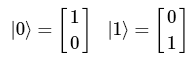
\includegraphics[width=4cm]{orgonal_vector.png}\\\textit{Orthogonal Vectors}
\end{minipage}
\end{center}
\end{figure}
\subsection{Entanglement}
Entanglements gives quantum computing the ability to scale exponentially. If one qubit simultaneosly represents two states, two qubits represents four states when coupled together. They can no longer be treated independently, they now form a coupled or entangled, super state. As more qubits link together, the number of states exponentially increase, which could lead to a computer with astronomically large computing power.
\subsection{Fragility}
Quantum states are quite fragile. If you measure, observe, touch ot peturb any of these states, they collapse to a classical state. The states don't stick around for very long, which is why quantum computers are currently hard to build.
\subsection{No cloning}
A corrollary to fragility is the "No cloning theorem". In classical physics, if we have two bits, one can copy or eavesdrop and recreate the information. In contrast, the information entangled within a set of qubits will be lost if someone tries to observe or copy them. A quantum state cannot be copied without the sender or receiver realizing this. This concept serves as the basis of quantum communications.
\newpage
\section{Logic gates}
A logic gate is an idealized or physical device implementing a Boolean function, a logical operation performed on one or more binary inputs that produces a single binary output. 
Logic circuits include such devices as multiplexers, registers, arithmetic logic units (ALUs), and computer memory, all the way up through complete microprocessors, which may contain more than 100 million gates.
\subsection{Classical logic gates}
%--------------------------------------
\subsubsection{NOT}
\begin{figure}[h]
\begin{center}
\begin{minipage}[b]{4cm}
\centering
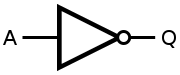
\includegraphics[width=2cm]{not_gate.png}\\\textit{NOT - gate}
\end{minipage}
\begin{minipage}[b]{2cm}
\centering
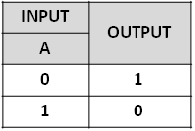
\includegraphics[width=2cm]{not_truthtable.png}\\\textit{NOT - Truth Table}
\end{minipage}
\end{center}
\end{figure}
%----------------------------------------
\subsubsection{AND}
\begin{figure}[h]
\begin{center}
\begin{minipage}[b]{4cm}
\centering
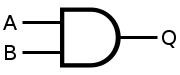
\includegraphics[width=2cm]{and_gate.png}\\\textit{AND - gate}
\end{minipage}
\begin{minipage}[b]{2cm}
\centering
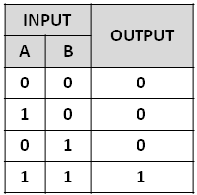
\includegraphics[width=2cm]{and_truthtable.png}\\\textit{AND - Truth Table}
\end{minipage}
\end{center}
\end{figure}
%--------------------------------------------
\subsubsection{OR}
\begin{figure}[h]
\begin{center}
\begin{minipage}[b]{4cm}
\centering
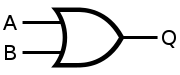
\includegraphics[width=2cm]{or_gate.png}\\\textit{OR - gate}
\end{minipage}
\begin{minipage}[b]{2cm}
\centering
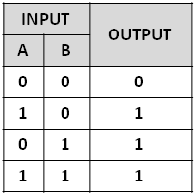
\includegraphics[width=2cm]{or_truthtable.png}\\\textit{OR - Truth Table}
\end{minipage}
\end{center}
\end{figure}
%--------------------------------------------
\newpage
\subsubsection{NAND}
\begin{figure}[h]
\begin{center}
\begin{minipage}[b]{4cm}
\centering
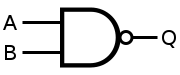
\includegraphics[width=2cm]{nand_gate.png}\\\textit{NAND - gate}
\end{minipage}
\begin{minipage}[b]{2cm}
\centering
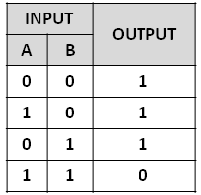
\includegraphics[width=2cm]{nand_truthtable.png}\\\textit{NAND - Truth Table}
\end{minipage}
\end{center}
\end{figure}
%--------------------------------------------
\subsubsection{NOR}
\begin{figure}[h]
\begin{center}
\begin{minipage}[b]{4cm}
\centering
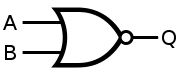
\includegraphics[width=2cm]{nor_gate.png}\\\textit{NOR - gate}
\end{minipage}
\begin{minipage}[b]{2cm}
\centering
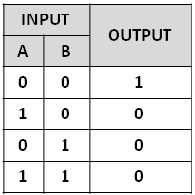
\includegraphics[width=2cm]{nor_truthtable.png}\\\textit{NOR - Truth Table}
\end{minipage}
\end{center}
\end{figure}
%--------------------------------------------
\subsubsection{XNOR}
\begin{figure}[h]
\begin{center}
\begin{minipage}[b]{4cm}
\centering
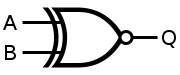
\includegraphics[width=2cm]{xnor_gate.png}\\\textit{XNOR - gate}
\end{minipage}
\begin{minipage}[b]{2cm}
\centering
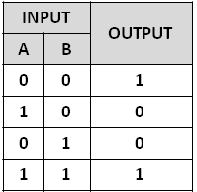
\includegraphics[width=2cm]{xnor_truthtable.png}\\\textit{XNOR - Truth Table}
\end{minipage}
\end{center}
\end{figure}
\newpage
%--------------------------------------------
\subsection{Quantum gates}
%------------------------------------------
\subsubsection{The X-Gate}
It simply flips the bit value: 0 becomes 1 and 1 becomes 0. For qubits, it is an operation called x that does the job of the NOT.
The X-gate is represented by the Pauli-X matrix.
Qbit negation is defined by the following transformations:
\begin{figure}[h]
\begin{center}
\begin{minipage}[b]{4cm}
\centering
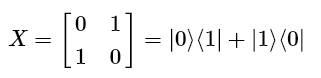
\includegraphics[width=4cm]{x_gate.png}\\\textit{The X-Gate}
\end{minipage}
\end{center}
\end{figure}
\begin{mdframed}
\begin{center}
\begin{minipage}[b]{4cm}
\centering
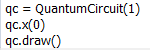
\includegraphics[width=4cm]{x_code.png}\\\textit{The X-Gate Code}
\end{minipage}
\begin{minipage}[b]{4cm}
\centering
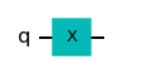
\includegraphics[width=4cm]{x_gate_schema.png}\\\textit{The X-Gate Schema}
\end{minipage}
\end{center}
\end{mdframed}
%---------------------------------------------
\subsubsection{The Y \& Z-gate }
Similarly to the X-gate, the Y \& Z Pauli matrices also act as the Y \& Z-gates:
\begin{figure}[h]
\begin{center}
\begin{minipage}[b]{4cm}
\centering
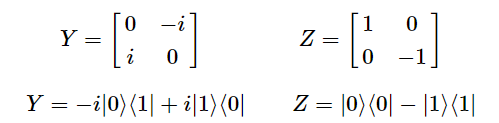
\includegraphics[width=6cm]{yandz_gate.png}\\\textit{The Y \& Z-Gate}
\end{minipage}
\end{center}
\end{figure}
\begin{mdframed}
\begin{center}
\begin{minipage}[b]{4cm}
\centering
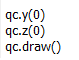
\includegraphics[width=2cm]{yandz_code.png}\\\textit{The Y \& Z-Gate Code}
\end{minipage}
\begin{minipage}[b]{4cm}
\centering
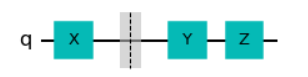
\includegraphics[width=4cm]{yandz_gate_schema.png}\\\textit{The Y \& Z-Gate Schema}
\end{minipage}
\end{center}
\end{mdframed}
%-------------------------------------------------
\subsubsection{The CNOT-gate } 
In quantum computers, the job of the XOR gate is done by the controlled-NOT gate. Since that's quite a long name, we usually just call it the CNOT. In Qiskit its name is cx, which is even shorter.
\begin{figure}[h]
\begin{center}
\begin{minipage}[b]{3cm}
\centering
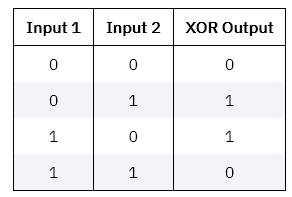
\includegraphics[width=3cm]{cnot_truthtable.png}\\\textit{The CNOT-gate Truth Table}
\end{minipage}
\end{center}
\end{figure}
\newpage
\begin{mdframed}
\begin{center}
\begin{minipage}[b]{4cm}
\centering
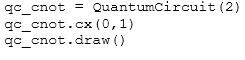
\includegraphics[width=4cm]{cnot_code.png}\\\textit{The CNOT-gate Code}
\end{minipage}
\begin{minipage}[b]{4cm}
\centering
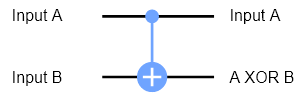
\includegraphics[width=4cm]{cnot_schema.png}\\\textit{The CNOT-gate Schema}
\end{minipage}
\end{center}
\end{mdframed}
%-------------------------------------------------
\subsubsection{The Toffoli-gate} 
This new gate is called the Toffoli. For those of you who are familiar with Boolean logic gates, it is basically an AND gate.
In Qiskit, the Toffoli is represented with the ccx command.
\begin{mdframed}
\begin{center}
\begin{minipage}[b]{4cm}
\centering
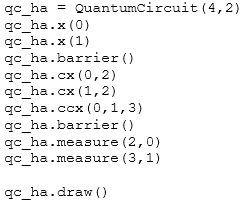
\includegraphics[width=4cm]{toffoli_code.png}\\\textit{The Toffoli-gate Code}
\end{minipage}
\begin{minipage}[b]{5cm}
\centering
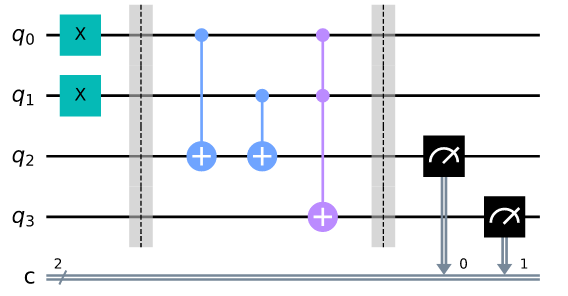
\includegraphics[width=5cm]{toffoli_schema.png}\\\textit{The Toffoli-gate Schema}
\end{minipage}
\end{center}
\end{mdframed}
%-------------------------
\subsubsection{The Hadamard-gate} 
The Hadamard gate (H-gate) is a fundamental quantum gate. It allows us to move away from the poles of the Bloch sphere and create a superposition of |0⟩ and |1⟩. 
\begin{figure}[h]
\begin{center}
\begin{minipage}[b]{4cm}
\centering
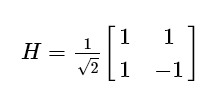
\includegraphics[width=4cm]{hadamard_gate.png}\\\textit{The Hadamard-gate}
\end{minipage}
\begin{minipage}[b]{5cm}
\centering
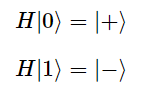
\includegraphics[width=3cm]{hadamard_gate_transformation.png}\\\textit{The hadamard-gate}
\end{minipage}
\end{center}
\end{figure}
%-------------------------
\newpage
\section{Deutsch algorithm}
The Deutsch-Jozsa algorithm, was the first example of a quantum algorithm that performs better than the best classical algorithm. 
There is given a hidden Boolean function f, which takes as input a string of bits, and returns either 0 or 1, that is:
\begin{figure}[h]
\begin{center}
\begin{minipage}[b]{4cm}
\centering
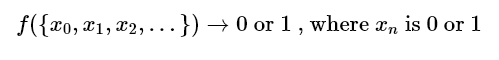
\includegraphics[width=6cm]{deutch_boolean.png}\\\textit{The boolean function}
\end{minipage}
\end{center}
\end{figure}
\newline
The property of the given Boolean function is that it is guaranteed to either be balanced or constant. A constant function returns all 0's or all 1's for any input, while a balanced function returns 0's for exactly half of all inputs and 1's for the other half. 
The Deutch-Jozsa algorithm task is to determine whether the given function is balanced or constant.
This problem could be solve by quantum computer provided it has the function f implemented as a quantum oracle, which maps the state |x>|y> to state |x>|y$\oplus$f(x)> (where $\oplus$ is addition modulo 2).
\newline Below is the generic circuit for the Deutsch-Jozsa algorithm.
\begin{figure}[h]
\begin{center}
\begin{minipage}[b]{4cm}
\centering
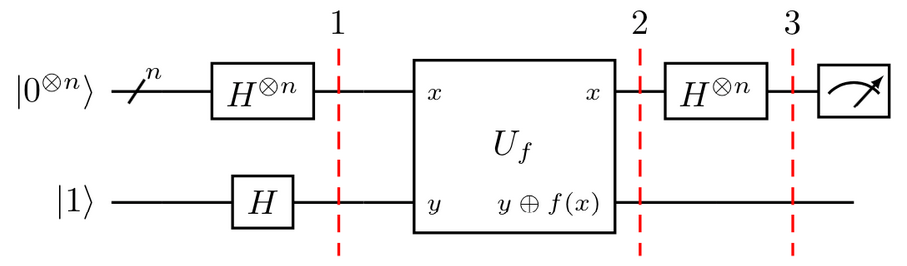
\includegraphics[width=8cm]{deutch_schema.png}\\\textit{The generic circuit for the Deutch-Jozsa algorithm}
\end{minipage}
\end{center}
\end{figure}
\newline
The steps of the algorithm:
\begin{enumerate}[start=1]
\item Prepare two quantum registers. The first is an n-qubit register initialized to |0⟩, and the second is a one-qubit register initialized to |1⟩.
\item Apply a Hadamard gate to each qubit.
\item Apply the quantum oracle |x⟩|y⟩ to |x⟩|y$\oplus$f(x)⟩.
\item Apply a Hadamard gate to each qubit in the first register.
\item Measure the first register. Notice that the probability of measuring which evaluates to 1 if f(x) is constant and 0 if f(x) is balanced.
\newline
When the oracle is constant, it has no effect on the input qubits, and the quantum states before and after querying the oracle are the same. 
When the oracle is balanced, phase kickback adds a negative phase to exactly half states.
The quantum state after querying the oracle is orthogonal to the quantum state before querying the oracle. Thus, in Step 4, when applying the H-gates, we must end up with a quantum state that is orthogonal to |00…0⟩. This means we should never measure the all-zero state.
\end{enumerate}
\newpage
%bibligrafia
%\section*{Bibliography}
\begin{thebibliography}{x}
  % \bibitem{<biblabel>} <citation>
  \bibitem{citeA}
    {\scshape Mark Oskin}, {\itshape Quantum Computing - Lecture Notes}
  \bibitem{citeB}
    {\scshape David McMahon}, {\itshape Quantum Computing Explained}, A John Wiley \& Sons, Inc., Publication, 2007.
   \bibitem{citeC}
    {\scshape quiskit.org}, {\itshape Qiskit 0.36.2 documentation}
\addcontentsline{toc}{section}{References}
\end{thebibliography}
\end{document}
%-------------------------------------------------
